% =====================================================================
% Plantilla de respuestas · Tarea Computacional · IMT2220 (2026-2)
% =====================================================================
% Cómo usarla:
%   1. Completen el número de grupo y los integrantes (más abajo).
%   2. Reemplacen cada \pendiente por su desarrollo y su respuesta.
%   3. Las figuras que guarden desde sus notebooks van en la carpeta figuras/.
%   4. Compilen con pdfLaTeX (en Overleaf es el compilador por defecto) o con LuaLaTeX.
%
% En Overleaf: New Project > Upload Project y suban el .zip con esta carpeta.
% Pueden borrar estos comentarios y las cajas de "Indicaciones" cuando terminen.
\documentclass{article}
\usepackage{plantilla}
\graphicspath{{figuras/}}
\settitulo{Tarea Computacional}

% ---------------------------------------------------------------------
% Datos del grupo
% ---------------------------------------------------------------------
\newcommand\grupo{10}
\integrantes{%
  Lucas Martín Chicao Carmona \\
  Ignacio Andrés Osorio Orellana \\
  Martín Ignacio Serrano Pizarro \\
  Martin Antonio Von Gehr Campos\par}

% Marca para lo que falta por completar (búsquenla con Ctrl+F antes de entregar)
\newcommand\pendiente{{\color{gris90}\itshape [Escriban aquí su desarrollo y su respuesta.]}}

% \figura[ancho]{archivo}{leyenda}{etiqueta}: incluye figuras/archivo. Mientras el notebook no la
% haya generado, muestra un recuadro en su lugar (búsquenlo con Ctrl+F: "Falta") y el informe compila.
\newcommand\figura[4][\linewidth]{%
  \begin{figure}[H]
    \centering
    \IfFileExists{figuras/#2}%
      {\includegraphics[width=#1]{#2}}%
      {\fbox{\parbox{0.8\linewidth}{\centering\itshape\color{gris90}
        [Falta \code{figuras/\detokenize{#2}}: se genera al ejecutar el notebook.]}}}
    \caption{#3}
    \label{#4}
  \end{figure}}

\begin{document}

\portada[Grupo \grupo]

% =====================================================================
\seccionsinnumero{Indicaciones para usar esta plantilla}
% =====================================================================

\begin{nota}[Indicaciones]
  Esta plantilla es recomendada para resolver la tarea (aunque pueden utilizar cualquier otro formato mientras cumplan con lo solicitado). 
  Pueden reemplazar cada \pendiente{} por su desarrollo.
  Al final de este archivo hay ejemplos de cómo escribir ecuaciones, incluir figuras y tablas. Borren esa página antes de entregar.
\end{nota}

Algunas recomendaciones
\begin{itemize}
  \item \textbf{Desarrollo.} Justifiquen cada paso: no basta con el resultado. Cuando usen un resultado de clases, menciónenlo.
  \item \textbf{Resultados numéricos.} Reporten los valores que se piden (normas, residuos, $J(\theta)$, etc.) con 3 o 4 cifras significativas e indiquen de qué celda del notebook salen. (Esto no es estrictamente necesario, pero sí recomendado.)
  \item \textbf{Figuras.} Guárdenlas desde el notebook con \code{plt.savefig("figuras/nombre.png", dpi=200, bbox\_inches="tight")}, súbanlas a la carpeta \code{figuras/} (para que puedan añadirlas aquí) y comenten lo que se ve en ellas.
\end{itemize}
\despueslista

% =====================================================================
\problema{Reconstrucción de una imagen}
% =====================================================================

\seccion{(a) Mínimos cuadrados}

\begin{enumerate}[label=\roman*., widest=iii]
  \item \textbf{Gradiente y matriz Hessiana de $J_0$.}

  \pendiente

  \item \textbf{$H_{J_0}$ es semidefinida positiva y todo punto crítico es un mínimo global.}

  \pendiente

  \item \textbf{Unicidad o infinitos minimizadores.}

  \pendiente
\end{enumerate}
\despueslista

\seccion{(b) Reconstrucción}

\begin{enumerate}[label=\roman*., widest=ii]
  \item \textbf{Implementación.} Reporten $\norm{x_0}_2$, $\max_i \abs{x_{0,i}}$ y $\norm{Ax_0 - b}_2$, muestren lado a lado $b$ y $x_0$, y respondan las preguntas.

  \figura[0.6\linewidth]{P1_b_reconstruccion.png}{Imagen observada $b$ y solución directa $x_0$.}{fig:p1b}

  \pendiente

  \item \textbf{Explicación.}

  \pendiente
\end{enumerate}
\despueslista

\seccion{(c) Regularización de Tikhonov}

\begin{enumerate}[label=\roman*., widest=iv]
  \item \textbf{Gradiente, Hessiana y único minimizador global.}

  Expandiendo la norma,
  \[
    J_\lambda(x) = x^T A^T A x - 2 (A^T b)^T x + b^T b + \lambda x^T x,
  \]
  y derivando se obtiene
  \[
    \nabla J_\lambda(x) = 2A^T(Ax - b) + 2\lambda x, \qquad H_{J_\lambda} = 2(A^T A + \lambda I).
  \]
  Para cada vector propio $v_i$ de $A^T A$ se tiene $H_{J_\lambda} v_i = 2(\mu_i + \lambda) v_i$. Como $v_1, \dots, v_n$ es una base ortonormal de $\R^n$, los valores propios de $H_{J_\lambda}$ son exactamente $2(\mu_i + \lambda)$. Además,
  \[
    \mu_i = v_i^T A^T A v_i = \norm{Av_i}_2^2 \geq 0,
  \]
  por lo que $2(\mu_i + \lambda) \geq 2\lambda > 0$ y $H_{J_\lambda}$ es definida positiva.

  La matriz $A^T A + \lambda I$ tiene valores propios $\mu_i + \lambda > 0$, luego es invertible y la ecuación $\nabla J_\lambda(x) = 0$, es decir $(A^T A + \lambda I)x = A^T b$, tiene como única solución
  \[
    x_\lambda = (A^T A + \lambda I)^{-1} A^T b.
  \]
  Como $J_\lambda$ es un polinomio de grado 2, su aproximación de Taylor de segundo orden es exacta. Usando $\nabla J_\lambda(x_\lambda) = 0$ y que $H_{J_\lambda}$ es definida positiva, para todo $y \neq x_\lambda$ resulta
  \[
    J_\lambda(y) - J_\lambda(x_\lambda) = \tfrac{1}{2}(y - x_\lambda)^T H_{J_\lambda} (y - x_\lambda) > 0.
  \]
  Por lo tanto, $x_\lambda$ es el único minimizador global de $J_\lambda$.

  \item \textbf{Descomposición de $\ip{x_\lambda}{v_i}$ y cota del aporte del ruido.}

  Tomamos producto interno con $v_i$ en $(A^T A + \lambda I) x_\lambda = A^T b$. Como $A^T A + \lambda I$ es simétrica y $v_i$ es vector propio,
  \[
    (\mu_i + \lambda)\ip{x_\lambda}{v_i} = \ip{A^T b}{v_i} = \ip{b}{Av_i},
  \]
  donde la última igualdad usa que $\ip{u}{w} = u^T w$ y que $(A^T b)^T = b^T A$. Reemplazando $b = Ax^* + \eta$ y usando $\ip{Ax^*}{Av_i} = \ip{x^*}{A^T A v_i} = \mu_i \ip{x^*}{v_i}$, se obtiene
  \[
    \ip{x_\lambda}{v_i} = \frac{\mu_i}{\mu_i + \lambda}\ip{x^*}{v_i} + \frac{\ip{Av_i}{\eta}}{\mu_i + \lambda}.
  \]
  Para la cota usamos Cauchy-Schwarz y $\norm{Av_i}_2 = \sqrt{\mu_i}$:
  \[
    \abs*{\frac{\ip{Av_i}{\eta}}{\mu_i + \lambda}} \leq \frac{\sqrt{\mu_i}}{\mu_i + \lambda}\norm{\eta}_2 \leq \frac{\norm{\eta}_2}{2\sqrt{\lambda}},
  \]
  donde la última desigualdad es la indicación $\mu_i + \lambda \geq 2\sqrt{\mu_i \lambda}$ si $\mu_i > 0$, y es inmediata si $\mu_i = 0$.

  Los números $\ip{x_\lambda}{v_i}$ son las coordenadas de $x_\lambda$ en la base $v_1, \dots, v_n$. El primer término depende solo de la imagen verdadera: es la coordenada $\ip{x^*}{v_i}$ multiplicada por el factor $\mu_i/(\mu_i + \lambda) \in [0, 1)$, y es lo único que quedaría si no hubiera ruido. El segundo depende solo de $\eta$ y no de $x^*$, por lo que es el aporte del ruido. A diferencia de (b), donde el error en la dirección $v_i$ solo se podía acotar por $\norm{\eta}_2/\sqrt{\mu_i}$, que explota cuando $\mu_i \to 0$, ahora la cota no depende de $\mu_i$.

  \item \textbf{Interpretación.}

  El comportamiento lo determina el factor $\mu_i/(\mu_i + \lambda)$:
  \begin{itemize}
    \item Si $\mu_i \gg \lambda$, el factor es cercano a 1 y $\ip{x_\lambda}{v_i} \approx \ip{x^*}{v_i} + \ip{Av_i}{\eta}/\mu_i$. La componente de $x^*$ se recupera casi intacta y el error, acotado por $\norm{\eta}_2/\sqrt{\mu_i}$, es pequeño porque $\mu_i$ es grande.
    \item Si $\mu_i \ll \lambda$, el factor es cercano a 0. La componente de $x^*$ se pierde, pero el aporte del ruido también se atenúa, pues está acotado por $\sqrt{\mu_i}\norm{\eta}_2/\lambda$.
  \end{itemize}
  Así, $\lambda$ actúa como un umbral: se conservan las direcciones que el desenfoque preserva y se descartan aquellas en las que el ruido dominaría.

  Si $\lambda$ es muy pequeño, casi todos los factores valen 1 y $x_\lambda$ se aproxima a $x_0$, con el ruido amplificado en las direcciones de $\mu_i$ pequeño. Si $\lambda$ es muy grande, todos los factores se acercan a 0, por lo que $x_\lambda \to 0$: el ruido desaparece, pero también la imagen, que resulta borrosa y oscura, y el residuo tiende a $\norm{b}_2$.

  \item \textbf{Implementación.} Los valores se obtienen en la celda de (c) iv del notebook.

  \begin{table}[H]
    \centering
    \begin{tabular}{>{\filatabla}l c c}
      \toprule[0.8bp]
                           & $\norm{x}_2$ & $\norm{Ax - b}_2$ \\
      \midrule[0.4bp]
      $x_0$                & $3{,}503 \times 10^{5}$ & $6{,}71 \times 10^{-12}$ \\
      $\lambda = 10^{-3.5}$ & $37{,}06$ & $0{,}5617$ \\
      $\lambda = 10^{-2.5}$ & $36{,}02$ & $0{,}6169$ \\
      $\lambda = 1$        & $17{,}18$ & $17{,}85$ \\
      \bottomrule[0.8bp]
    \end{tabular}
    \caption{Norma y residuo de cada reconstrucción.}
    \label{tab:ridge}
  \end{table}

  \figura{P1_c_tikhonov.png}{Imagen observada $b$, solución directa $x_0$ y reconstrucciones $x_\lambda$ para $\lambda \in \{10^{-3.5}, 10^{-2.5}, 1\}$.}{fig:p1c}

  Como no tiene sentido ajustar $b$ mejor que el tamaño del ruido, comparamos cada residuo con $\delta = 0{,}64$:
  \begin{itemize}
    \item $x_0$: el residuo es $6{,}71 \times 10^{-12} \ll \delta$, es decir, $x_0$ ajusta también el ruido. Su norma, $3{,}503 \times 10^{5}$, es muy superior al máximo posible de 64 y la imagen no contiene información reconocible.
    \item $\lambda = 10^{-3.5}$: el residuo es $0{,}5617 \approx 0{,}88\,\delta$. La norma ya es razonable y aparece la estructura de la imagen, pero con mucho grano: las direcciones con $\mu_i$ cercano a $\lambda$ siguen dejando pasar ruido, y la cota de (c) ii vale $\delta/(2\sqrt{\lambda}) \approx 18{,}0$. Además, $\max_i \abs{x_i} = 1{,}178$ se sale del intervalo $[0, 1]$.
    \item $\lambda = 10^{-2.5}$: el residuo es $0{,}6169 \approx 0{,}96\,\delta$, el más cercano a $\delta$. La cota del ruido baja a $\approx 5{,}69$, los valores se mantienen en el rango ($\max_i \abs{x_i} = 0{,}9618$) y la imagen se ve nítida y con poco grano.
    \item $\lambda = 1$: el residuo es $17{,}85 \approx 27{,}9\,\delta$, muy superior al ruido, por lo que se está regularizando de más. Como $\norm{Ax}_2 \leq \norm{x}_2$, se tiene $\mu_i = \norm{Av_i}_2^2 \leq 1$, y entonces todos los factores cumplen $\mu_i/(\mu_i + 1) \leq 1/2$: incluso las componentes mejor conservadas se reducen a la mitad o menos. Esto explica que la imagen resulte borrosa y oscura, con $\max_i \abs{x_i} = 0{,}4171$.
  \end{itemize}
  La mejor reconstrucción de las tres es la de $\lambda = 10^{-2.5}$, que equilibra la imagen recuperada con el ruido admitido, tal como predicen (c) ii y iii.
\end{enumerate}
\despueslista

\seccion{(d) Píxeles dañados}

Sea $\tilde{x}_\lambda = (A^T A + \lambda I)^{-1} A^T \tilde{b}$ la reconstrucción de Tikhonov a partir de $\tilde{b}$.

\figura[0.6\linewidth]{P1_d_danados.png}{Observación $\tilde{b}$ con píxeles dañados y su reconstrucción de Tikhonov con $\lambda = 10^{-2.5}$.}{fig:p1d}

Con $\lambda = 10^{-2.5}$, la reconstrucción no muestra ninguna estructura reconocible: se obtiene $\norm{\tilde{x}_\lambda}_2 = 45{,}91$, $\max_i \abs{\tilde{x}_{\lambda,i}} = 2{,}395$, fuera del intervalo $[0, 1]$, y $\norm{A\tilde{x}_\lambda - \tilde{b}}_2 \approx 10$.

\begin{enumerate}[label=\roman*., widest=iii]
  \item \textbf{$\tilde{\eta} = \eta + (\tilde{b} - b)$ e interpretación de sus sumandos.}

  De $\tilde{b} = Ax^* + \tilde{\eta}$ y $Ax^* = b - \eta$ se obtiene
  \[
    \tilde{\eta} = \tilde{b} - Ax^* = \tilde{b} - b + \eta = \eta + (\tilde{b} - b).
  \]
  El sumando $\eta$ es el ruido habitual del sensor: pequeño y repartido en todos los píxeles, con $\norm{\eta}_2 \approx \delta$. El sumando $\tilde{b} - b$ es el error causado por los píxeles dañados: vale cero en los píxeles sanos y, en los dañados, es la diferencia entre la lectura correcta y el valor 0 o 1 que quedó registrado.

  \item \textbf{$\norm{\tilde{b} - b}_2$ y comparación de $\norm{\tilde{\eta}}_2$ con $\delta$.}

  En los datos, 430 de los 4096 píxeles (10,5\,\%) valen exactamente 0 o 1, y en todos los demás $\tilde{b}$ coincide con $b$. Se obtiene
  \[
    \norm{\tilde{b} - b}_2 = 10{,}74,
  \]
  con diferencias de hasta $0{,}8225$ en un píxel. Como $\eta$ no se conoce, $\norm{\tilde{\eta}}_2$ no se puede calcular de forma exacta, pero la desigualdad triangular aplicada a $\tilde{\eta} = \eta + (\tilde{b} - b)$ y a $\tilde{b} - b = \tilde{\eta} - \eta$, junto con $\norm{\eta}_2 \approx \delta$, entrega
  \[
    10{,}10 \lesssim \norm{\tilde{\eta}}_2 \lesssim 11{,}38.
  \]
  Es decir, $\norm{\tilde{\eta}}_2$ es entre 16 y 18 veces mayor que $\delta = 0{,}64$. El nuevo ruido está dominado por los píxeles dañados.

  \item \textbf{¿Por qué fracasa la reconstrucción? ¿Bastaría con aumentar $\lambda$?}

  La deducción de (c) ii solo usa que $\tilde{b} = Ax^* + \tilde{\eta}$, de modo que
  \[
    \ip{\tilde{x}_\lambda}{v_i} = \frac{\mu_i}{\mu_i + \lambda}\ip{x^*}{v_i} + \frac{\ip{Av_i}{\tilde{\eta}}}{\mu_i + \lambda}, \qquad \abs*{\frac{\ip{Av_i}{\tilde{\eta}}}{\mu_i + \lambda}} \leq \frac{\norm{\tilde{\eta}}_2}{2\sqrt{\lambda}}.
  \]
  Con $\lambda = 10^{-2.5}$ la cota pasa de $\approx 5{,}69$ a un valor entre $90$ y $101$. El valor de $\lambda$ que funcionaba para un ruido de tamaño $\delta$ ya no controla un ruido unas 17 veces mayor, y el segundo término pasa a dominar sobre la imagen. Además, $J_\lambda$ trata todas las lecturas por igual, por lo que no tiene forma de distinguir las lecturas erróneas de las correctas.

  Aumentar $\lambda$ no basta. Para que la cota vuelva a su valor anterior habría que multiplicar $\lambda$ por $(\norm{\tilde{\eta}}_2/\delta)^2 \approx 280$, es decir, llegar a $\lambda \approx 0{,}9$. Eso es prácticamente el caso $\lambda = 1$ de (c) iv, en el que ningún factor $\mu_i/(\mu_i + \lambda)$ supera $1/2$ y la imagen queda borrosa y oscura.

  Como $x^*$ no se conoce, en la Tabla~\ref{tab:danados} usamos como referencia $x_\lambda$ con $\lambda = 10^{-2.5}$, obtenida desde $b$ en (c) iv. Aumentar $\lambda$ ayuda solo hasta cierto punto: la distancia a la referencia baja de $28{,}5$ a $8{,}45$ en $\lambda = 10^{-1.5}$, cuyo residuo, $10{,}35$, ya es del orden de $\norm{\tilde{\eta}}_2$. Pero esa imagen conserva manchas producidas por los píxeles dañados (Figura~\ref{fig:p1dlambda}). Al seguir aumentando $\lambda$ las manchas se atenúan, pero la distancia vuelve a crecer y la imagen pierde detalle y brillo. Ningún valor de $\lambda$ probado se acerca a la calidad obtenida sin píxeles dañados, porque $\lambda$ reduce el ruido y la imagen al mismo tiempo.

  \begin{table}[H]
    \centering
    \begin{tabular}{>{\filatabla}l c c c}
      \toprule[0.8bp]
      & $\norm{\tilde{x}_\lambda}_2$ & $\norm{\tilde{x}_\lambda - x_{10^{-2.5}}}_2$ & $\norm{A\tilde{x}_\lambda - \tilde{b}}_2$ \\
      \midrule[0.4bp]
      $\lambda = 10^{-2.5}$ & $45{,}91$ & $28{,}5$ & $10{,}0$ \\
      $\lambda = 10^{-1.5}$ & $35{,}61$ & $8{,}45$ & $10{,}35$ \\
      $\lambda = 10^{-0.5}$ & $26{,}61$ & $10{,}46$ & $13{,}73$ \\
      $\lambda = 1$         & $17{,}16$ & $19{,}3$ & $20{,}73$ \\
      \bottomrule[0.8bp]
    \end{tabular}
    \caption{Reconstrucciones desde $\tilde{b}$ al aumentar $\lambda$, comparadas con $x_{10^{-2.5}}$, obtenida desde $b$.}
    \label{tab:danados}
  \end{table}

  \figura{P1_d_lambda.png}{Referencia obtenida desde $b$ y reconstrucciones desde $\tilde{b}$ para valores crecientes de $\lambda$.}{fig:p1dlambda}
\end{enumerate}
\despueslista

\seccion{(Bonus) Mínimos cuadrados ponderados}

\figura[0.6\linewidth]{P1_bonus_ponderados.png}{Reconstrucción de Tikhonov a partir de $\tilde{b}$ y reconstrucción con mínimos cuadrados ponderados.}{fig:p1bonus}

\pendiente

% =====================================================================
\problema{Red neuronal con dos capas ocultas}
% =====================================================================

\seccion{(a) Derivada de la sigmoide}

Calculamos la derivada de $\sigma(t)$ usando la regla del cociente:
\begin{align*}
  \sigma'(t) &= \frac{d}{dt}\left(\frac{1}{1 + e^{-t}}\right)
    = \frac{\frac{d}{dt}(1) \cdot (1 + e^{-t}) - (1) \cdot \frac{d}{dt}(1 + e^{-t})}{(1 + e^{-t})^2} \\[4pt]
  &= \frac{(0)(1 + e^{-t}) - (1) \cdot \left(\frac{d}{dt}(1) + \frac{d}{dt}(e^{-t})\right)}{(1 + e^{-t})^2} \\[4pt]
  &= \frac{(-1) \cdot \left(0 + e^{-t} \cdot \frac{d}{dt}(-t)\right)}{(1 + e^{-t})^2} \\[4pt]
  &= \frac{(-1) \cdot \left(e^{-t} \cdot (-1)\right)}{(1 + e^{-t})^2}
    = \frac{e^{-t}}{(1 + e^{-t})^2}.
\end{align*}
Sumando y restando 1 en el numerador, se obtiene:
\begin{align*}
  \sigma'(t) &= \frac{1 + e^{-t} - 1}{(1 + e^{-t})^2}
    = \frac{1 + e^{-t}}{(1 + e^{-t})^2} - \frac{1}{(1 + e^{-t})^2} \\[4pt]
  &= \frac{1}{1 + e^{-t}} - \frac{1}{(1 + e^{-t})^2}
    = \frac{1}{1 + e^{-t}} \left(1 - \frac{1}{1 + e^{-t}}\right) \\[4pt]
  &= \sigma(t) \, (1 - \sigma(t)).
\end{align*}

Dado que la función sigmoide se define como:
\begin{align*}
\sigma(t) = \frac{1}{1 + e^{-t}}
\end{align*}

se cumple $e^{-t} > 0$ para todo $t \in \mathbb{R}$, lo cual implica que:
\begin{align*}
0 < \sigma(t) < 1, \quad \forall t \in \mathbb{R}
\end{align*}
A partir de $\sigma'(t) = \sigma(t)(1 - \sigma(t))$, deducimos directamente que:
\begin{align*}
\sigma'(t) > 0 \quad \forall t \in \mathbb{R}
\end{align*}

Necesitamos encontrar el valor máximo de $\sigma'(t)$, tal que realizaremos el cambio de variable $u = \sigma(t) \in (0,1)$ y definiremos la función:
\begin{align*}
g(u) = u(1 - u) = u - u^2
\end{align*}

Derivando $g(u)$ con respecto a $u$ e igualando a cero para encontrar sus puntos críticos:
\begin{align*}
g'(u) = 1 - 2u = 0 \implies u = \frac{1}{2}
\end{align*}

Dado que la segunda derivada de $g(u)$ es $g''(u) = -2 < 0$, el punto $u = 1/2$ corresponde a un máximo global en el intervalo $(0,1)$. Evaluando $g(u)$ en este punto:
\begin{align*}
g\left(\frac{1}{2}\right) = \frac{1}{2}\left(1 - \frac{1}{2}\right) = \frac{1}{4}
\end{align*}

Por lo tanto, se concluye que:
\begin{align*}
0 < \sigma'(t) \le \frac{1}{4} \quad \forall t \in \mathbb{R}
\end{align*}


Luego, el valor máximo de $\sigma'(t)$ se alcanza cuando $\sigma(t) = \frac{1}{2}$. Resolviendo para $t$:
\begin{align*}
\sigma(t) = \frac{1}{1 + e^{-t}} = \frac{1}{2} \implies 1 + e^{-t} = 2 \implies e^{-t} = 1 \implies t = 0
\end{align*}

Así, la derivada $\sigma'$ alcanza su máximo global en $t = 0$, tal que $\sigma'(0) = \frac{1}{4}$.

\end{align*}

% Falta: deducir que 0 < sigma'(t) <= 1/4 para todo t y en qué punto se alcanza el máximo.


\seccion{(b) Función de pérdida y su gradiente}
Necesitamos calcular $\nabla_\theta \mathcal{J}(\theta)$, usando el error individual $e_i = \hat{y}_i - y_i$ 
y siguiendo el camino por el que cada parámetro afecta a $\mathcal{L}_i = \frac{1}{2}e_i^2$ 
aplicando la regla de la cadena, tenemos:

\nabla_\theta \mathcal{J}(\theta) 
= \frac{1}{N} \sum_{i=1}^{N} \nabla_\theta \mathcal{L}_i(\theta)
= \frac{1}{N} \sum_{i=1}^{N}
\begin{pmatrix}
\dfrac{\partial \mathcal{L}_i}{\partial a_1} \\[10pt]
\dfrac{\partial \mathcal{L}_i}{\partial b_1} \\[10pt]
\dfrac{\partial \mathcal{L}_i}{\partial a_2} \\[10pt]
\dfrac{\partial \mathcal{L}_i}{\partial b_2} \\[10pt]
\dfrac{\partial \mathcal{L}_i}{\partial v}   \\[10pt]
\dfrac{\partial \mathcal{L}_i}{\partial c}
\end{pmatrix}

Para cada componente seguimos el camino desde el parámetro hasta $\mathcal{L}_i$:

\begin{align*}
\frac{\partial \mathcal{L}_i}{\partial c}
&= \frac{\partial \mathcal{L}_i}{\partial \hat{y}_i}
   \cdot \frac{\partial \hat{y}_i}{\partial c}
 = e_i \cdot 1
 = e_i \\[10pt]
\frac{\partial \mathcal{L}_i}{\partial v}
&= \frac{\partial \mathcal{L}_i}{\partial \hat{y}_i}
   \cdot \frac{\partial \hat{y}_i}{\partial v}
 = e_i \cdot h_{2,i} \\[10pt]
\frac{\partial \mathcal{L}_i}{\partial b_2}
&= \frac{\partial \mathcal{L}_i}{\partial \hat{y}_i}
   \cdot \frac{\partial \hat{y}_i}{\partial h_{2,i}}
   \cdot \frac{\partial h_{2,i}}{\partial z_{2,i}}
   \cdot \frac{\partial z_{2,i}}{\partial b_2}
 = e_i \cdot v \cdot \sigma'(z_{2,i}) \cdot 1 \\[10pt]
\frac{\partial \mathcal{L}_i}{\partial a_2}
&= \frac{\partial \mathcal{L}_i}{\partial \hat{y}_i}
   \cdot \frac{\partial \hat{y}_i}{\partial h_{2,i}}
   \cdot \frac{\partial h_{2,i}}{\partial z_{2,i}}
   \cdot \frac{\partial z_{2,i}}{\partial a_2}
 = e_i \cdot v \cdot \sigma'(z_{2,i}) \cdot h_{1,i} \\[10pt]
\frac{\partial \mathcal{L}_i}{\partial b_1}
&= \frac{\partial \mathcal{L}_i}{\partial \hat{y}_i}
   \cdot \frac{\partial \hat{y}_i}{\partial h_{2,i}}
   \cdot \frac{\partial h_{2,i}}{\partial z_{2,i}}
   \cdot \frac{\partial z_{2,i}}{\partial h_{1,i}}
   \cdot \frac{\partial h_{1,i}}{\partial z_{1,i}}
   \cdot \frac{\partial z_{1,i}}{\partial b_1}
 = e_i \cdot v \cdot \sigma'(z_{2,i}) \cdot a_2 \cdot \sigma'(z_{1,i}) \cdot 1 \\[10pt]
\frac{\partial \mathcal{L}_i}{\partial a_1}
&= \frac{\partial \mathcal{L}_i}{\partial \hat{y}_i}
   \cdot \frac{\partial \hat{y}_i}{\partial h_{2,i}}
   \cdot \frac{\partial h_{2,i}}{\partial z_{2,i}}
   \cdot \frac{\partial z_{2,i}}{\partial h_{1,i}}
   \cdot \frac{\partial h_{1,i}}{\partial z_{1,i}}
   \cdot \frac{\partial z_{1,i}}{\partial a_1}
 = e_i \cdot v \cdot \sigma'(z_{2,i}) \cdot a_2 \cdot \sigma'(z_{1,i}) \cdot x_i
\end{align*}
Por lo tanto:
\nabla_\theta \mathcal{J}(\theta)
= \frac{1}{N} \sum_{i=1}^{N}
\begin{pmatrix}
e_i \, v \, \sigma'(z_{2,i}) \, a_2 \, \sigma'(z_{1,i}) \, x_i\\
e_i \, v \, \sigma'(z_{2,i}) \, a_2 \, \sigma'(z_{1,i})\\
e_i \, v \, \sigma'(z_{2,i}) \, h_{1,i}\\
e_i \, v \, \sigma'(z_{2,i})\\
e_i \, h_{2,i}\\
e_i
\end{pmatrix}



\seccion{(c) Implementación y verificación del gradiente}



\begin{table}[H]
  \centering
  \begin{tabular}{>{\filatabla}c r r r}
    \toprule[0.8bp]
    Parámetro & Fórmula de (b) & $D_j$ & Diferencia \\
    \midrule[0.4bp]
    $a_1$ & $3{,}17 \times 10^{-4}$ & $3{,}17 \times 10^{-4}$ & $2{,}72 \times 10^{-12}$ \\
    $b_1$ & $-1{,}23 \times 10^{-3}$ & $-1{,}23 \times 10^{-3}$ & $1{,}31 \times 10^{-11}$ \\
    $a_2$ & $-2{,}83 \times 10^{-3}$ & $-2{,}83 \times 10^{-3}$ & $1{,}74 \times 10^{-11}$ \\
    $b_2$ & $-9{,}49 \times 10^{-3}$ & $-9{,}49 \times 10^{-3}$ & $1{,}38 \times 10^{-11}$ \\
    $v$   & $-5{,}95 \times 10^{-1}$ & $-5{,}95 \times 10^{-1}$ & $8{,}97 \times 10^{-12}$ \\
    $c$   & $-1{,}58$                & $-1{,}58$                & $2{,}79 \times 10^{-12}$ \\
    \bottomrule[0.8bp]
  \end{tabular}
  \caption{Gradiente en $\theta_0$: fórmulas de (b) y diferencias centradas.}
  \label{tab:gradiente}
\end{table}
* -1.58 se obtuvo como -1.58e+00 pero se decidió anotar así en vez de $-1{,}58 \times 10^{0}$



El vector inicial es

\[

  \theta_0 = (0{,}912;\ {-0{,}585};\ 0{,}657;\ {-0{,}701};\ 0{,}026;\ {-0{,}728}),

  \qquad J(\theta_0) = 1{,}6229.
\]

El error máximo entre el gradiente obtenido y las diferencias centradas es

$E = 1{,}74 \times 10^{-11} 

\seccion{(d) Descenso del gradiente}

\figura[0.7\linewidth]{P2_d_error.png}{Evolución de $J(\theta_k)$ con $\alpha = 1$.}{fig:p2d}

La Figura 5 muestra $J(\theta_k)$ en escala logarítmica. La pérdida cae rápidamente durante las primeras (aproximadamente) 2000 iteraciones y luego se estabiliza gradualmente, luego de estas iteraciones la curva se vuelve casi lineal, convergiendo a un valor minimo de costo constante.





\seccion{(e) Parámetros encontrados}


\figura[0.7\linewidth]{P2_e_ajuste.png}{Datos de entrenamiento y curva $x \mapsto \hat{y}(x; \theta_{20.000})$ en $[-1, 1]$.}{fig:p2e}

Tras 20\,000 iteraciones con $\alpha = 1$ se obtiene

\[

  \theta_{20000} = (4{,}623;\ 0{,}718;\ 4{,}394;\ {-0{,}990};\ {-3{,}178};\ 3{,}086),

  \qquad J(\theta_{20000}) = 1{,}395 \times 10^{-3}.

\]

Como se observa en la Figura 6, la curva $x \mapsto \hat{y}(x;\theta_{20000})$ ajusta bien los datos, siguiendo una forma decreciente que va desde aproximadamente $y = 2.1$, hasta aproximadamente $y = 0$.





\seccion{(f) Sensibilidad del entrenamiento}

\begin{enumerate}[label=\roman*., widest=ii]
  \item \textbf{Tamaño del paso.}

  \figura[0.7\linewidth]{P2_f_pasos.png}{Curvas de error para $\alpha \in \{0{,}01;\ 0{,}1;\ 1;\ 2{,}5\}$, partiendo del mismo $\theta_0$.}{fig:p2fi}

  Los valores finales de $J$ para cada paso son:

  \begin{itemize}

    \item $\alpha = 0{,}01$: $J_{20000} = 0{,}1265$. El paso es demasiado pequeño, entonces el algoritmo converge muy lentamente y en 20000 iteraciones no alcanza un mínimo de calidad comparable.

    \item $\alpha = 0{,}1$: $J_{20000} = 1{,}404 \times 10^{-3}$. Converge bien aunque más lento que $\alpha=1$.

    \item $\alpha = 1$: $J_{20000} = 1{,}395 \times 10^{-3}$. Es el paso más eficiente, dado que converge rápido y alcanza el menor valor de $J$.

    \item $\alpha = 2{,}5$: $J$ deja de ser finito en la iteración $k = 8$. El paso es demasiado grande y en cada actualización los parámetros crecen de manera descontrolada hasta que rapidamente ocurre desbordamiento numérico (\textit{overflow}).

  \end{itemize}

  En resumen, un paso muy pequeño ralentiza la convergencia, mientras que un paso excesivamente grande provoca divergencia. El valor $\alpha = 1$ resulta el más adecuado para este problema.




  \item \textbf{Distintas inicializaciones.}

  \figura[0.8\linewidth]{P2_f_inicializaciones.png}{Valores finales de $J$ para 10 inicializaciones con componentes en $[-1, 1]$ y 10 con componentes en $[-5, 5]$.}{fig:p2fii}

Con inicializaciones en $[-1,1]$, las 10 inicializaciones obtienen valores de $J$ finales parecidos, lo que sugiere que el descenso del gradiente encuentra consistentenmente un buen minimo sin importar el punto de partida. En cambio en $[-5,5]$, algunas inicializaciones quedan atascadas y terminan con valores de $J$ ligeramente superiores al resto. Esto puede deberse a que cuando los parametros iniciales son muy grandes en valor absoluto, los gradientes son casi cero desde el inicio ($\sigma'(t)\approx0$ cuando $\abs{t}$ es grande), por lo que el algrotitmo logra moverse muy poco apenas con cada iteración, y no logran alejarse del punto de partida desfavorable.
Esto también demuestra que el descenso del gradiente no garantiza encontrar el mínimo global, dado que dependiendo del punto de partida, se puede terminar llegando a un minimo local o a una zona plana de la cual es dificil desestancarse.

\end{enumerate}
\despueslista

\seccion{(g) Datos de otra función}

\begin{enumerate}[label=\roman*., widest=ii]
  \item \textbf{Entrenamiento.}

  \figura[0.7\linewidth]{P2_g_ajuste.png}{Datos $(x_i, \tilde{y}_i)$ y curva obtenida con la misma red.}{fig:p2g}

Entrenando con \texttt{datos\_P2\_g.csv} desde el mismo $\theta_0$ con $\alpha=1$ y 20000 iteraciones se obtiene $J = 7{,}822\times10^{-2}$, valor considerablemente mayor que el $1{,}395\times10^{-3}$ alcanzado con los datos originales. Como muestra la Figura 9, la curva ajustada no logra seguir la forma de los datos $\tilde{y}_i$. Esto se explica en el item siguiente.


  \item \textbf{Monotonía, cotas y por qué la red no puede aproximar $\tilde{f}$.}
  
Calculamos la derivada de $\hat{y}(x; \theta)$ respecto de $x$ aplicando la regla de la cadena:
\[
\frac{d\hat{y}}{dx} = v \cdot \sigma'(z_2) \cdot a_2 \cdot \sigma'(z_1) \cdot a_1
\]

Como $\sigma'(t) > 0$ para todo $t \in \mathbb{R}$, el signo de $d\hat{y}/dx$ coincide con el de $v \cdot a_1 \cdot a_2$, el cual es constante respecto a $x$. Por tanto, $x \mapsto \hat{y}(x; \theta)$ es una función \textbf{monótona} en $\mathbb{R}$ para cualquier $\theta \in \mathbb{R}^6$ (siendo estrictamente monótona si $v \cdot a_1 \cdot a_2 \neq 0$).

Respecto a las cotas, como $0 < \sigma(t) < 1$ para todo $t \in \mathbb{R}$, se tiene que $0 < h_2 < 1$ y por lo tanto:
\[
\hat{y}(x; \theta) = c + v h_2 \in 
\begin{cases} 
(c, c + v) & \text{si } v > 0, \\
(c + v, c) & \text{si } v < 0, \\
\{c\} & \text{si } v = 0.
\end{cases}
\]
Es decir, los valores de $\hat{y}$ están siempre acotados estrictamente entre $c$ y $c + v$.
\\Observando los datos de \texttt{datos\_P2\_g.csv}, la función $\tilde{f}$ no es monótona, ya que aumenta para $x < 0$ y disminuye para $x > 0$. Dado que toda función representable por esta red es monótona, no existe ningún $\theta \in \mathbb{R}^6$ con el que la red pueda aproximar bien a $\tilde{f}$, sin importar la cantidad de iteraciones, $\alpha$ utilizado, ni la inicialización elegida. La red de una sola neurona por capa oculta restringe el espacio de funciones representables únicamente a las funciones monótonas.

\end{enumerate}

% =====================================================================
\clearpage\markright{}
\seccionsinnumero{Ejemplos de uso (borren esta sección antes de entregar)}
% =====================================================================

\seccion{Ecuaciones}

Una ecuación destacada se escribe entre \code{\textbackslash[} y \code{\textbackslash]}:
\[ \nabla J_0(x) = 2A^T(Ax - b). \]
Para varias líneas alineadas, usen \code{align*}:
\begin{align*}
  J_\lambda(x) &= \norm{Ax - b}_2^2 + \lambda \norm{x}_2^2 \\
               &= x^T (A^T A + \lambda I) x - 2 (A^T b)^T x + b^T b.
\end{align*}
La plantilla define \code{\textbackslash norm\{x\}}, \code{\textbackslash abs\{x\}}, \code{\textbackslash ip\{u\}\{v\}} (producto interno $\ip{u}{v}$), \code{\textbackslash R} ($\R$) y \code{\textbackslash diag}.

\seccion{Figuras}

Guarden la figura desde el notebook en la carpeta \code{figuras/} e inclúyanla así:
\begin{figure}[H]
  \centering
  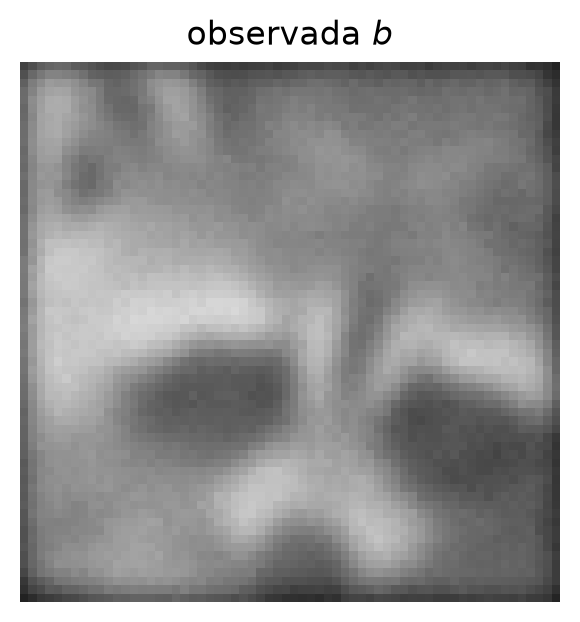
\includegraphics[width=6cm]{ejemplo_b.png}
  \caption{Imagen observada $b$ (ejemplo con los datos de la pauta).}
  \label{fig:ejemplo}
\end{figure}
Para referirse a ella, escriban \code{Figura\textasciitilde\textbackslash ref\{fig:ejemplo\}}: Figura~\ref{fig:ejemplo}.

\seccion{Cajas de comentarios}

\begin{nota}[Observación]
  Si quieren destacar un comentario, usen el entorno \code{nota}.
\end{nota}

\end{document}
